\section{Metode Konstruksi NFA: Algoritma Thompson}

Algoritma Thompson menyediakan template standar untuk mengubah setiap operator Regular Expression menjadi bagian dari NFA secara rekursif.

\subsection{Template Dasar Thompson}
\begin{itemize}
    \item \textbf{Literal (a)}: Transisi tunggal dari state awal ke akhir dengan simbol 'a'.
    \item \textbf{Union (R|S)}: Menggunakan $\epsilon$-transitions untuk bercabang ke NFA R dan NFA S secara paralel.
    \item \textbf{Concatenation (RS)}: Menghubungkan NFA R langsung ke NFA S melalui transisi $\epsilon$.
    \item \textbf{Kleene Star ($R^*$)}: Menambahkan loop balik $\epsilon$ dan jalur pintas $\epsilon$ untuk mengakomodasi pengulangan nol kali.
\end{itemize}

\begin{figure}[!htbp]
    \centering
    \adjustbox{max width=0.7\textwidth,center}{%
    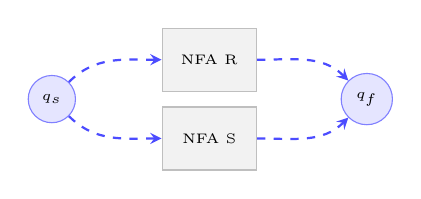
\begin{tikzpicture}[
        state/.style={circle, draw=blue!50, fill=blue!10, minimum size=0.6cm, font=\tiny},
        box/.style={rectangle, draw=gray!50, fill=gray!10, minimum width=1.2cm, minimum height=0.8cm, font=\tiny, align=center},
        arrow/.style={->, >=stealth, thick},
        eps/.style={->, >=stealth, thick, dashed, blue!70}
    ]
    \node[state] (q0) at (0,0) {$q_s$};
    \node[box] (R) at (2,0.5) {NFA R};
    \node[box] (S) at (2,-0.5) {NFA S};
    \node[state] (qf) at (4,0) {$q_f$};
    \draw[eps] (q0) to[out=45, in=180] (R);
    \draw[eps] (q0) to[out=-45, in=180] (S);
    \draw[eps] (R) to[out=0, in=135] (qf);
    \draw[eps] (S) to[out=0, in=-135] (qf);
    \end{tikzpicture}%
    }
    \caption{Template Thompson untuk Union ($R|S$)}
\end{figure}
